\chapter{Methodology}
\label{Method}

The process for predicting the portfolio load using graph classification is performed in several stages, an overview of which can be seen in Figure \ref{fig:ProcessFlow}. The following method is written in order to increase understanding of the project and aid reproducibility. The methodology developed in this chapter ensures that the resulting graphs are made in efficiently and that clustering maximises the modularity of each graph. Checks for the probability distributions are discussed to ensure that the findings are not due to spurious relationships in the data. Finally the models developed are discussed, and where appropriate, defined mathematically and the evaluation metrics discussed.

\begin{figure}[ht]
    \centering
    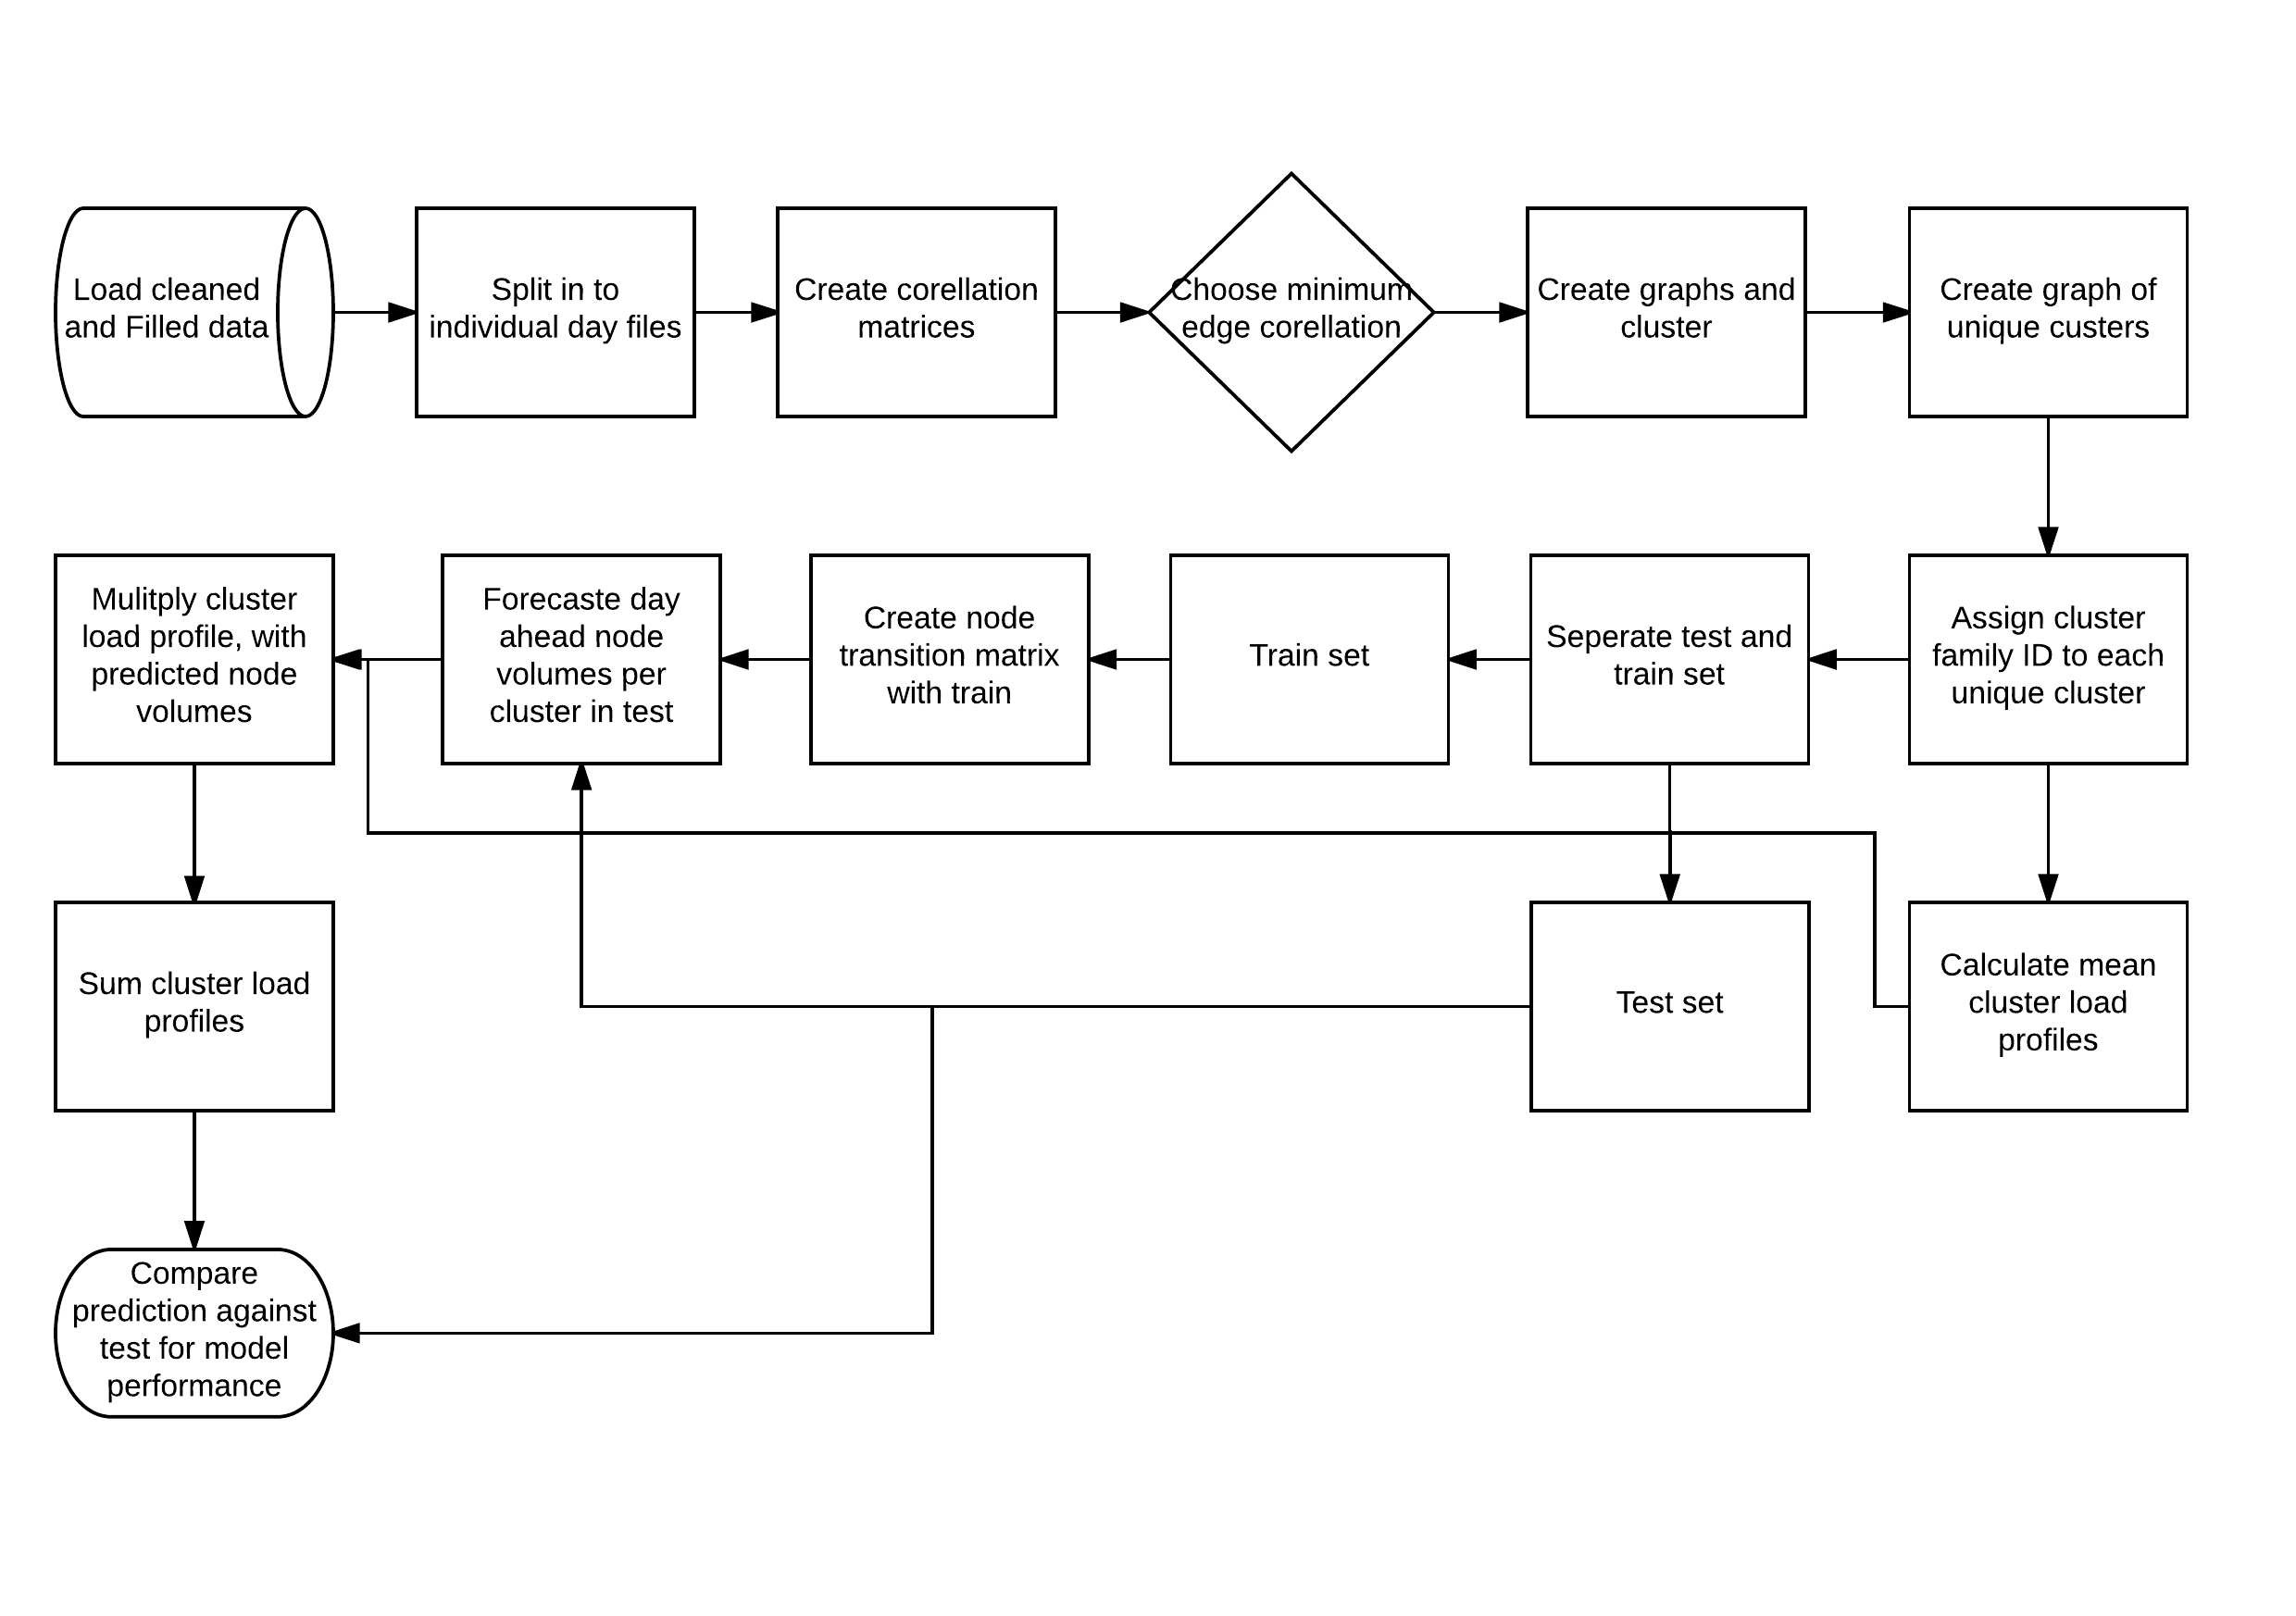
\includegraphics[width =\textwidth]{Figures/Appendix/Thesisprocess.png}
    \caption[Project process]{Flow chart showing the process of generating and testing the predictive model once the data has been cleaned}
    \label{fig:ProcessFlow}
\end{figure}


\section{Creating correlation matrices}
\label{sec:cormat} \label{sec:CormatEdge}
The graph building block is the similarity metric that forms the link between smart meters. As was shown in Section \ref{sec:basicconsum}, the distribution of power is not normal, meaning that Spearman's correlation \cite{spearmansrankcorrelationcoefficient2016} was preferred instead of Pearson's. Spearman's rho is a non-parametric test allowing for non-normal distributions, it uses ranks instead of raw scores. Two formulas for Spearman's correlation are shown in equations \ref{eq:spearmans1} to \ref{eq:spearmans3}, rank is shown by $rg_x$ and $rg_y$. Equation \ref{eq:spearmans1} is the base version of Spearman's rho whilst \ref{eq:spearmans2} is a version which can be used if the ranks are all distinct integers, in this project equation \ref{eq:spearmans1} is used.

As there are 5260 nodes in the dataset the resulting matrix contained 2.7 million elements, of varying degree's of correlation, the ordered correlation matrix for 09-08-2011 is shown in Figure \ref{fig:day100corplot}. By creating the correlation matrices for all days, it reduces the computational load for making changes later on in the processing pipeline, such as changing the minimum correlation requirements for link and rebuilding the graphs. Each correlation matrix was over 200mb, together the total size of all the correlation matrices was over 40Gb.

\begin{equation}
\label{eq:spearmans1}
    \rho = \frac{cov(rg_x,rg_y)}{\sigma_{rg_x}\sigma_{rg_y}}
\end{equation}

\begin{equation}
\label{eq:spearmans2}
    \rho = 1- \frac{6 \sum d_i^2}{n(n-1))}
\end{equation}

\begin{equation}
\label{eq:spearmans3}
    d_i = rg(X_i)-rg(Y_i)
\end{equation}

\begin{figure}
    \centering
    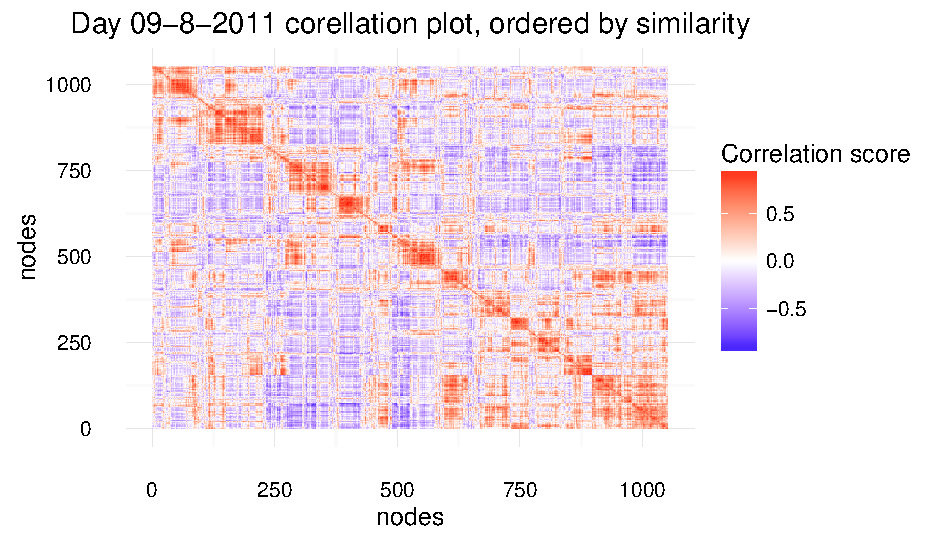
\includegraphics[width=\textwidth]{Figures/Results/day100Corplot}
    \caption[Example corellation matrix]{The correlation matrix of 09-08-2011 with the nodes organised by hierarchical similarity.}
    \label{fig:day100corplot}
\end{figure}


\section{Finding an appropriate  edge correlation cut off point}
As the dataset has 5260 nodes the the number of edges in a fully connected graph is almost 14 million which is intractable on a normal machine especially as the edges are weighted. It is also doubtful how much extra information will be gained using a fully connected graph instead of using a graph where the edges of the adjacency matrix is determined by a cut off distance. In order to measure the effect of a cut off value the number of edges and non isolated nodes were counted in each graph for a given correlation cut off, starting at 0.1 and increasing by 0.05 up to 1. In order to avoid constructing a large number of highly complex graphs the correlation matrices of each day were turned into logical matrices using the form $A>x$ where $A$ is the correlation matrix and $x$ is the cut off point, the number of isolated nodes is then equal to the number of rows/columns with a sum of 0 (the diagonal of the correlation matrix has already been set to zero).

The results of edge analysis are shown in Figure \ref{fig:EdgeNodeAnalysis}. They reveal that that the number of edges and non-isolated nodes are relatively consistent across the graphs. Sub Figure \ref{fig:Meanedges} shows that the number of edges decreases approximately quadratically with increasing minimum correlation. It can be seen that there is a small right skew in the data as there is a visible difference between the mean and the median, the standard deviation of the edge number is approximately 10\% of the mean. 

Sub Figure \ref{fig:Meannodes} shows the mean number of nodes for each cut off point. Node number analysis showed very little variation with a negligible standard deviation and a median that is the same as the mean. It is clear that the total number of non-isolated nodes stays almost constant up to quite high levels of correlation before dropping off steeply to zero. Comparing the percentage of non-isolated nodes against the percentage of total edges as in Figure \ref{fig:Edgenodeperc} shows that the percentage difference between the two grows quite large, Figure \ref{fig:EdgeNodeDiff} shows the difference is maximised at a cut off of 0.8. 

The results of this analysis suggests that using 0.8 as a cut off will provide the highest number of non-isolated nodes for the lowest number of edges. However it should be noted that although the number of non-isolated nodes is low, experimenting with various graphs reveals that there are many nodes in small unconnected sub graphs of two or three, therefore the cut off point will be set at a more conservative 0.7. This makes a much more highly connected graph but is still tractable. 

With the cut off point chosen at 0.7 all graphs can be generated and community detection performed.

\begin{figure*}[ht]
\centering
\textbf{Number of edges analysis}\par\medskip
\subfloat[]{
  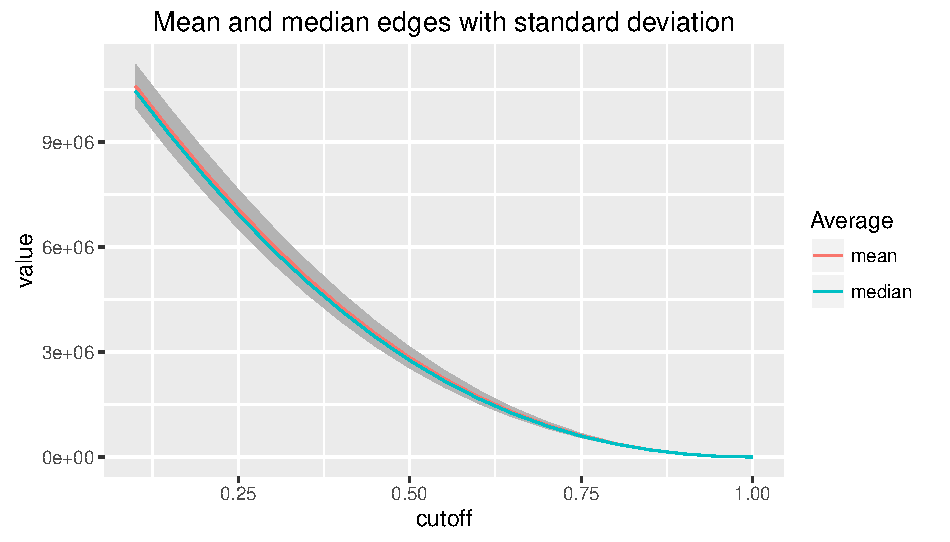
\includegraphics[width=0.49\textwidth]{Figures/Results/Meanedges}\label{fig:Meanedges}
}
\subfloat[]{
  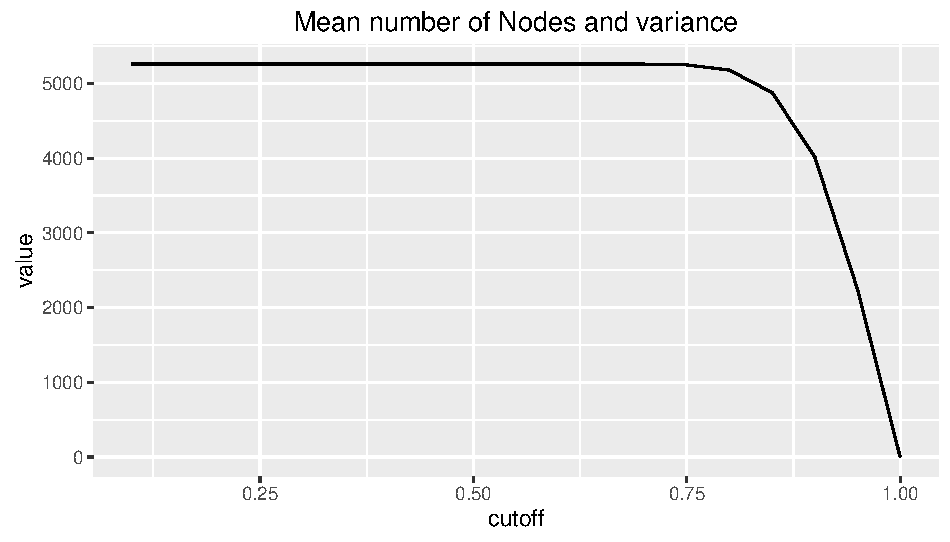
\includegraphics[width=0.49\textwidth]{Figures/Results/Meannodes}\label{fig:Meannodes}
}

\subfloat[]{
  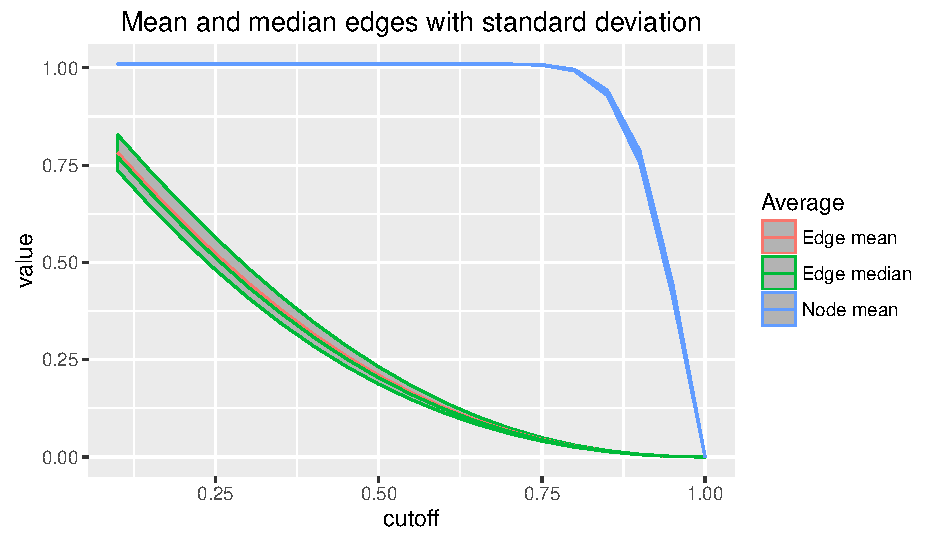
\includegraphics[width=0.49\textwidth]{Figures/Results/Edgenodeperc}\label{fig:Edgenodeperc}
}
\subfloat[]{
  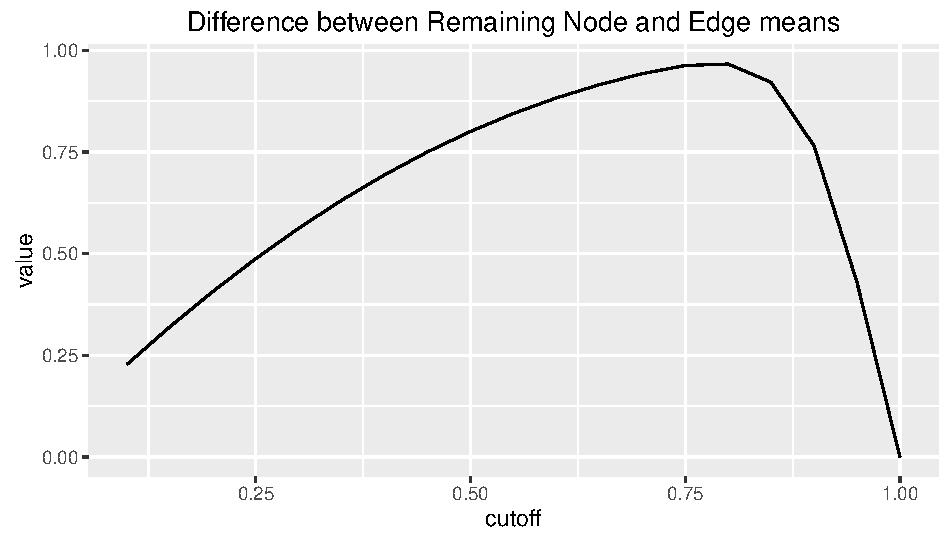
\includegraphics[width=0.49\textwidth]{Figures/Results/EdgeNodeDiff}\label{fig:EdgeNodeDiff}
}
\caption[Number of edges analysis]{Analysis of the number of edges and nodes for given correlation cut offs, across all 233 days, shows a relatively low standard deviation and slight skew with the number of edges. The number of nodes has an extremely low standard deviation, comparing the difference between the percentage remaining nodes and edges sees that the value is maximised at a correlation cut off of about 0.8. }
\label{fig:EdgeNodeAnalysis}
\end{figure*}



\subsection{Comparison with an Erdos-Renyi graph}
The Erdos-Renyi (ER) graph, developed by P Erdos and A Renyi in 1959 \cite{erdos1959}, showed that for any graph $\mathcal{G}$ had an equally likely probability of appearing when the number of vertices $v$ and edges $m$ were fixed, this is the so called GnM model, which is a graph $G$ with $n$ nodes and $M$ edges. In this model each element in the adjacency matrix has an equal probability of being present, that is $\frac{2m}{v(v-1)}$. In 1960 Erdos and Renyi explored the properties of the GnP \cite{erds1960}, which is a graph $G$ with $n$ nodes and each edge has an equal probability $P$. They found that above a critical level there was a high probability of the graph being connected (no isolated nodes) see equation \ref{eq:connected}. 

\begin{equation}
\label{eq:connected}
    p>\frac{(1+\epsilon)ln \; n }{n}
\end{equation}

An ER graph represents random noise, we will test whether the smart meter data has a significantly different number of isolated nodes than an ER graph for the same number of edges. If there is a significant difference between the graphs then it can be inferred that there smart node graphs are not random. This test will be done by generating 20 different ER graphs with the same number of edges as the mean number of edges for each cut off point for the smart meter data. The mean number of non-isolated nodes will then be compared with the mean number from the smart meter data using a paired \textit{t}-test.

\begin{figure}
    \centering
    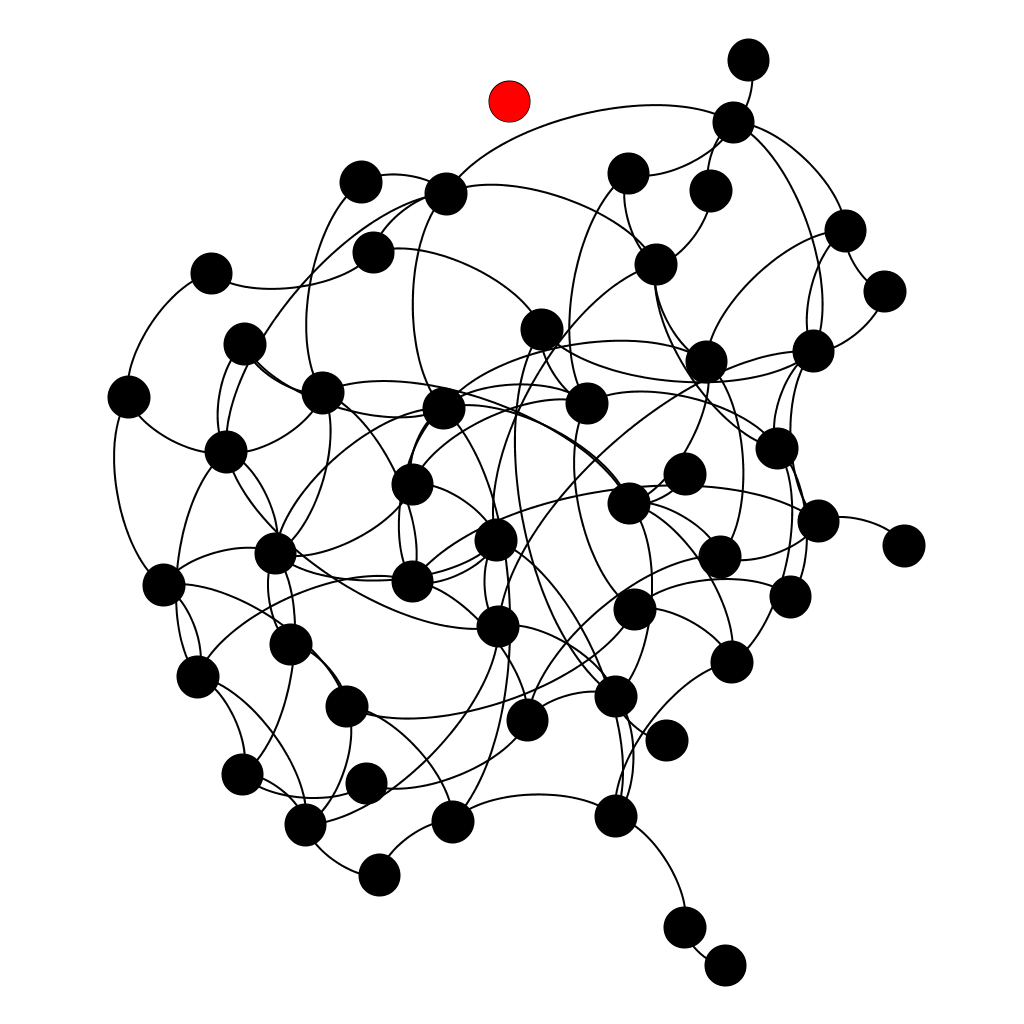
\includegraphics{Figures/Method/RandomGraph}
    \caption[Example Erdos-Renyi Graph]{An example of an Erdos-Renyi graph, generated with 50 nodes and 100 edges, note that the node highlighted in red has no edges and is separated from the the rest of the graph, despite the fact that the conditions in equation \ref{eq:connected} have been met. }
    \label{fig:RandomGraph}
\end{figure}

\section{Creating the graphs}
\label{chap:creategraph}

The correlation between the nodes will be converted in to a distance using $\sqrt(2(1-\rho))$ as popularised by Mantegna \cite{mantegna1999} and then into a weighted undirected graph. This distance metric is chosen over other metrics, such as euclidean distance, Manhattan or any other choice as it has been previously applied in a a similar time based setting, and that correlation is an a conceptually intuitive way to measure similarities over time as opposed to, for example, 12 dimensional euclidean space.  Once in graph form Community detection will be performed. The community detection algorithm used will be The Louvain algorithm, it was chosen from 4 different methods Fast Greedy, Walktrap, Louvain and Infomap mentioned in sections \ref{sec:commdetect}. The choice was made by selecting 50 random graphs and performing clustering on them using the different methods and then inspecting the resulting modularity scores and run time results. The results of the test shown in Figure \ref{fig:ChooseAlg} shows that although the results are similar for Walktrap, Infomap and Louvain, Louvain has a much lower average runtime than the other algorithms, therefore the Louvian algorithm was chosen.

\begin{figure*}[ht]
\centering
\subfloat[]{
  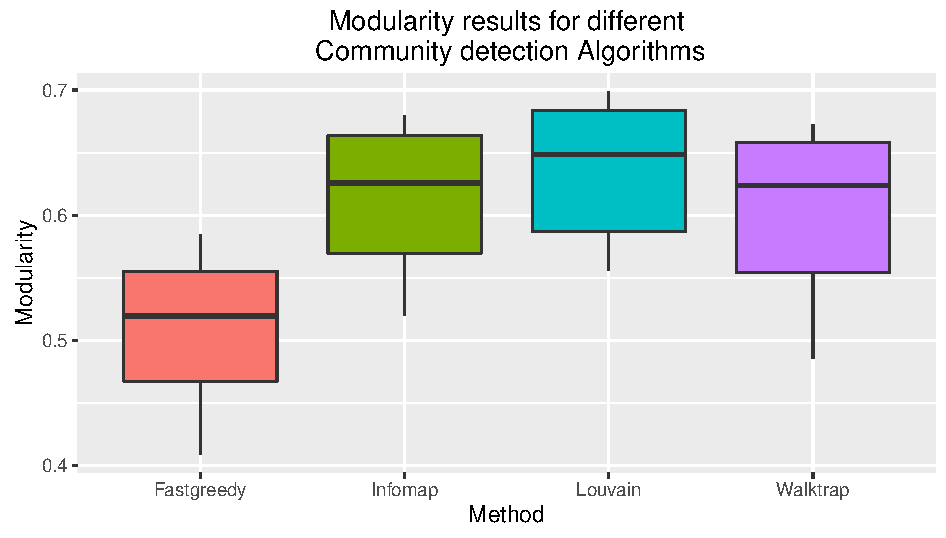
\includegraphics[width=0.80\textwidth]{Figures/Results/CommModComp}\label{fig:CommModComp}
}

\subfloat[]{
  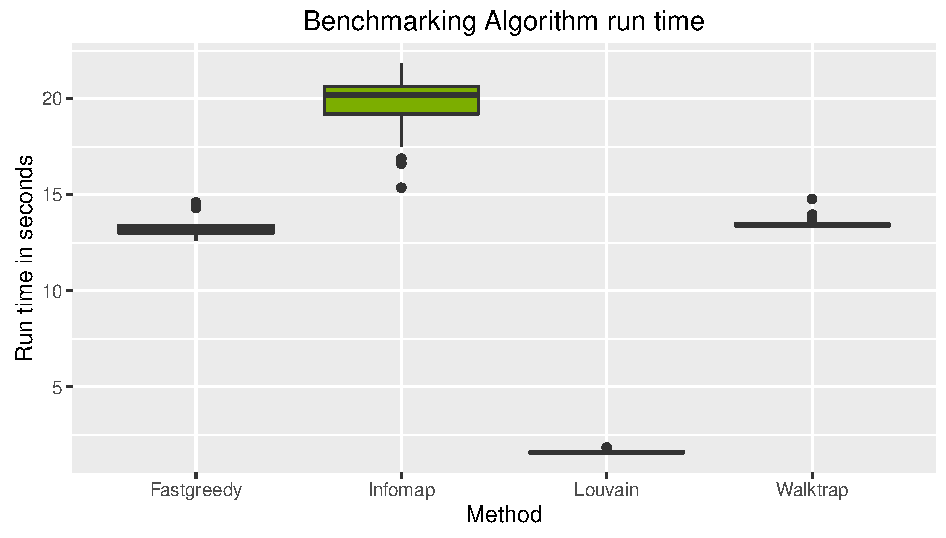
\includegraphics[width=0.80\textwidth]{Figures/Results/AlgorithmTimes}\label{fig:Algtime}
}

\caption[Cluster Family Load Profiles]{ Benchmarking the four target algorithms, shows that Walktrap, Infomap, and Louvain are all statistically similar in performance with Louvain getting slightly better results, however Louvain is considerably faster when it comes to detecting clusters}
\label{fig:ChooseAlg}
\end{figure*}

\section{Labelling clusters}
\label{sec:labelClust}

The result of the graph creation process will be 246 correlation matrices and corresponding graph structures, each graph will have a different number of clusters of different sizes and the clusters will all have slightly different profiles across days. This leads to the labelling problem of how to group various different but similar items into a set of finite groups when the group labels are unknown. In order to find our which clusters are similar to each other, and are part of the same cluster family the mean load profile of each cluster will be found and the same process used to discover the clusters discussed in Section \ref{sec:cormat} and \ref{chap:creategraph}, this will create clusters of clusters that will form the cluster families used to identify consistent behaviour types throughout the period.  The main difference will be that the cut off for the creation of a link will be set higher due to the inherently higher levels of correlation that will be present in the clusters, due to the averaging effect of clustering. This Process will create an $\mathbf{C_f}x\mathbf{C_f}$ correlation matrix where $\mathbf{C_u}$ is the total number of unique clusters across all days. 

In the creation of clusters not all nodes will behave similarly, certain clusters will appear only once, or contain a very small number of nodes, these clusters create noise which does not provide any value. To prevent a situation with a large number of clusters where only a small number are useful a "Node Soup" will be created. This soup will form a cluster of all clusters that contain either less than 50 nodes, or whose cluster family contains less than 1\% of the total node volume across the whole time frame.


\subsection{Load profiles}
\label{sec:LoadProfiles}
Once nodes have been assigned to clusters the load profile of each cluster can be calculated, four metrics will be used for visualisation of the cluster families and individual clusters and will define their characteristics and the common behaviour of the group as a whole. For the prediction part of the project the mean profile will be used as this has the advantage that the product of the mean load profile and the number of nodes in that cluster summed across all clusters is equal to the total load profile.

\begin{enumerate}
\itemsep0em 
\item Sum: The total kWh used by the cluster
\item Mean: The mean kWh of the nodes in the cluster
\item Median: The median kWh of the nodes in the cluster
\item Variance: The variance of the kWh of the nodes in the cluster
\end{enumerate}

\section{Probability distributions}

\subsection{Cluster transition}
\label{sec:Clusttrans}
An important stage of exploring how energy is consumed is by looking at the probability of nodes transitioning from one cluster to another across consecutive days. This analysis will create a transition matrix like that shown in Table \ref{tab:trans}, it can also be shown in graph form as in Figure \ref{fig:exampletrans}. 

\begin{table}[ht]
\centering
\begin{tabular}{|l|llll|} \hline
   & $c_1$  & $c_2$  & $c_3$  & $c_4$  \\ \hline
$c_1$ & 0.5 & 0   & 0   & 0.5 \\
$c_2$ & 0   & 0.8 & 0.2 & 0   \\
$c_3$ & 0   & 0.2 & 0.7 & 0.1   \\
$c_4$ & 0   & 0   & 0.1   & 0.9  \\ \hline
\end{tabular}
\caption[Example Cluster Transition matrix]{The transition matrix shows how a possible cluster transition could look. cluster $c_1$ will eventually be consumed by $c_4$. $c_2$ and $c_3$ have a constant low level exchange between each other. $c_4$ and $c_3$ also have a low level of exchange which means that $c_4$ will pass on some of the nodes it consumes from $c_1$ to $c_3$ and indirectly to $c_2$.}
\label{tab:trans}

\end{table}


\begin{figure}[ht]
\centering
  \includestandalone{Tikz/exampletrans1}
  \caption[Example cluster transition graph]{Graph showing an example of average transition of nodes between clusters each time step.}
  \label{fig:exampletrans}
\end{figure}

The transition matrix will be made using the following process. A matrix will be created with columns representing the unique clusters across all days and each row representing the unique Node ID's. An element is 1 if the node was present in that cluster and zero otherwise. Squaring the resulting binary matrix, such that $\mathbf{C_u^2}=\mathbf{C_u^t} \cdot \mathbf{C_u}$ where $\mathbf{C_u}$  is the number of unique clusters, will produce a matrix that is the sum of intersecting nodes from one Unique cluster to another. However the majority of the elements will need to be discarded as a Unique cluster can only transfer to a cluster in the subsequent day, it cannot be transferred to any days further foreword in time, it's own day or to any days in the past.

To resolve this problem a binary mask will be applied converting all invalid nodes to 0 and keeping all other elements the same. An example of such a mask can seen in Figure \ref{fig:ClusterMask}. After the mask has been applied only valid transfers will remain, the matrix will then be aggregated by cluster family to shrink the matrix to a $\mathbf{C_f} \cdot \mathbf{C_f}$ where $\mathbf{C_f}$ is the total number of cluster families including the Soup. The aggregated matrix will then represent the counts of node transfer from one cluster to another across all days. Dividing each row by it's total will create a probabilistic matrix similar to \ref{tab:trans}.

\begin{figure}
    \centering
    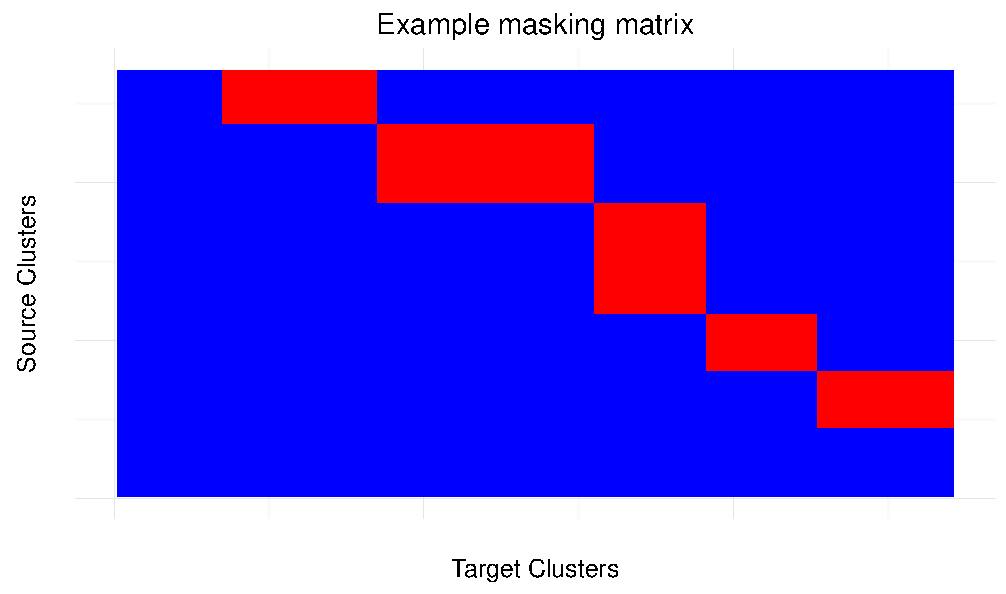
\includegraphics[width = \textwidth]{Figures/Method/ClusterMask}
    \caption[Cluster Transition Mask]{The figures shows an example mask that removes invalid Cluster transitions from the calculation of the transition matrix, note that the valid blocks sit just above the matrix diagonal. }
    \label{fig:ClusterMask}
\end{figure}

\begin{figure}[ht]
\centering
  \includestandalone{Tikz/continuationmergesplit}
  \caption[Cluster Continuation. Merge and Split]{The schematic shows a possible series of time steps where clusters $c_1$ and $c_2$ persist for three turns with little change before $c_1$ splits with most of it's nodes going to $c_2$ and the remainder forming a new node $c_3$. The arrows entering and leaving each node are nodes joining or leaving the cluster from the node soup of unattached nodes. N.B not all nodes are assigned to the two surviving clusters, some are lost to the node soup.}
  \label{fig:contmergsplit}
\end{figure}


\subsection{Node-cluster probability tables}
\label{sec:NodeClustProb}

With the Cluster families identified, creating a bi-variate conditional probability table to see the probability of a node being in a given cluster is of interest.  This is done by aggregating the matrix of Node cluster membership by cluster family so that each column represents the total number of days a node was in each of the cluster families. Dividing the rows of resulting matrix by the total row count will produce the bi-variate probability distribution. Each element of the resulting table will represent the conditional of a specific cluster given the node of interest $P(C_f|n)$, where $n$ is the node/smart meter of interest and $C_f$ is the cluster family.

\section{Analysing probability distributions}

With the creation of the transition matrix and the Node-Cluster probability table, it is instructive to see how much information can be gained from them. A simple method of doing this is to see how stable the nodes are in the clusters. For $C_f$ clusters the uniform probability of being in a cluster will be $\frac{1}{C_f}$. By squaring the elements and summing the rows, a uniform distribution will return a value of $\frac{1}{C_f}$ whilst a node that occurs in a single node only would return a value of 1. Plotting the density distribution will give a visualisation of how far from the uniform the bi-variate distribution is.

\subsection{Entropy and the KL divergence}
Although the Node stability method gives rough visual guide it can be more instructive to use the entropy of the distribution. Entropy is a measure of the uncertainty of a distribution, where a high value indicates a high uncertainty and an entropy of 0 is absolute certainty. A uniform distribution has the maximum entropy of a distribution as knowing $x$ gives zero information about the state of $y$, for a discrete distribution the entropy is always positive. Entropy itself is linked to two other concepts, the Kullback-Leibler divergence (KL-divergence) \cite{kullback1951} , and mutual information \cite{barber2012}. The KL-divergence is a measure of the similarity of two distributions and links to entropy as shown in \ref{eq:kl} where $H(p)$ is the entropy of the distribution $p$, whilst $u$ is the uniform distribution. The KL divergence is subtracted from the constant as it is always greater than or equal to zero, being zero when the two distributions are identical. The proof of that $KL(p|q)>0$ is shown in equations \ref{eq:klproofstart} to \ref{eq:klproofend}. The lowest level of useful entropy will be the marginal probability of being in a cluster i.e the probability distribution $P(C_f)$ for all values of $f$.

\begin{equation}
H(p)=-KL(p|u)+const
\label{eq:kl}
\end{equation}

 The KL divergence between 2 distributions $q(x)$ and $p(x)$ is defined as

\begin{equation}
    KL(q|p)= \left \langle log\, q(x) \right \rangle_{q(x)}-\left \langle log\, p(x) \right \rangle_{q(x)}
\label{eq:klproofstart}
\end{equation}

where $\left \langle f(x) \right \rangle$ means taking the expectation of function $f(x)$ with respect to the distribution $q(x)$.

consider the bound $log\, x \geq x-1$ show how this can be used to prove $KL(q|p)\geq0$.

\begin{equation}
    x = \frac{p(x)}{q(x)}
\end{equation}

Substitute into the bound equality
\begin{equation}
   log\,p(x)-log\,q(x) \geq \frac{p(x)}{q(x)}-1 
\end{equation}

multiply both sides by $q(x)$

\begin{equation}
    q(x)log\,p(x)-q(x)log\,q(x) \geq p(x)-q(x) 
\end{equation}

integrate both sides with respect to $x$ using the distribution property $\int q(x)dx=1 \,and \,\int p(x)dx=1 $

\begin{equation}
    \left \langle log\, q(x) \right \rangle_{q(x)}-\left \langle log\, p(x) \right \rangle_{q(x)} \geq 1-1
\end{equation}


\begin{equation}
    \left \langle log\, q(x) \right \rangle_{q(x)}-\left \langle log\, p(x) \right \rangle_{q(x)} \geq 0
\label{eq:klproofend}
\end{equation}

\subsection{Chi Squared test for independence}
A good method to test whether the two variables/axis of a  matrix are independent is to perform a Pearson $\chi^2$ independence test \cite{pearson1900}, shown. $O_i$ the number of observations of type $i$, $E_i$ is the expected frequency of type $i$ \cite{pearsonschisquaredtest2016}.

\begin{equation}
    \chi ^2 = \sum_{i=1}^n \frac{(O_i-E_i)^2}{E_i}
\end{equation}

\section{Modelling}
The main modelling approach in this project is to explore whether the method that predict the transition of nodes from one behavioural cluster to another can be used as a competitive forecasting technique when compared to a linear predictor and to see if it is in the ball park accuracy of the MAPE values obtained in the literature \ref{sec:forcesmart}, this regression model will output a single value for each half hour period that will be the prediction of the the electrical load for the whole domestic portfolio. It will be compared against a linear model that predicts using only the whole portfolio data ignoring the detail of the smart meters.

A secondary model will evaluate the ability of the transition matrix to correctly classify individual node movements instead of the en masse node flows of the main model, this classification model will predict which cluster the node will be in for the subsequent day. Whilst the comparison model of the regression will be a simple multi-linear regression, the classifier will be compared using the using the XGboost algorithm \cite{chen2016}. XGboost is a popular non-linear machine learning algorithm. The name refers to Extreme Gradient Boosting, as it is a development of earlier boosting techniques \cite{schapire2003} and boosted tree models, that were greatly popularised by Adaboost  \cite{freund1997}. However XGboost has been designed to use less resources and therefore have much greater scalability, than earlier boosting methods.

Finally a classification model will be used to take advantage of the socio-economic information available in the dataset, this model will attempt to predict socio-economic class based on electricity consumption patterns.


\subsection{Power forecasting}
The forecasting of the day ahead power will be done indirectly. A vector of the number of nodes in each cluster on day $x$ will be multiplied by the transition matrix developed in Section \ref{sec:Clusttrans} to predict the number of nodes in each cluster in day $x+1$, this will create a 1 step markov chain \cite{barber2012}. The mean node profiles of day $x$,mentioned in Section \ref{sec:LoadProfiles}, will then be multiplied by the predicted number nodes in each cluster of $x+1$, to create the predicted load profile of $x+1$. The concept with this modelling approach is that the amount of energy consumed in a domestic setting is driven by environmental factors such as temperature and light  \cite{hmgovernment2014} \cite{homesshowgreatestseasonalvariationinelectricityusetodayinenergyusenergyinformationadministrationeia2013}, as shown by the seasonal variation in Figure \ref{fig:DailyConsumption}. Therefore across neighbouring days the pattern of how and individual consumes energy would remain relatively constant but the number of people in each cluster would change based on behavioural patterns of getting home from work, evening clubs, movie night etc.
The model is defined in equations \ref{eq:begindef} to \ref{eq:enddef}, the accompanying text gives a descriptive explanation of the model and terms. for clarity a simple example using a 4 clusters and 3 time periods is show in equations \ref{eq:begineaxmple} to \ref{eq:endeaxmple}

The predicted number of nodes $\hat{N}_{x+1}$ are the product of the transition matrix $C_t$ and the number of nodes in each cluster $N_x$, where $C_t$ has dimensions $C_f \times C_f$ and $N_x$ is $C_f \times 1$ where $C_f$ is the total number of clusters.
\begin{equation}
C_t \:N_x=\hat{N}_{x+1}
\label{eq:begindef}
\end{equation}

The predicted load profile $\hat{L}_{x+1}$ is a matrix of dimensions $C_f\times t$ where $t$ is the number of time periods, in this case 12 for each half hour between 1630 and 2130, each row of the matrix represents the load profile of each cluster. $e_t$ is a vector of ones of length $1 \times t$. $\bar{L}_x$ a matrix of dimensions $C_f\times t$ where each row is the mean node load profile of each cluster on day $x$ measured in kWh. The predicted number of nodes per cluster is turned in into a matrix of dimension $C_f \times t$ by multiplying it by $e_t$, this produces a matrix where each column is the predicted nodes per cluster for day $x$ repeated $t$ times. This new matrix can then be multiplied element wise with $\bar{L}_x$ using the Hadamard product to find the predicted load per cluster.
\begin{equation}
\hat{N}_{x+1}\: e_t \circ \bar{L}_x=\hat{L}_{x+1}
\end{equation}

The total predicted load profile of $x+1$ calculated by summing the the predicted cluster loads using the vector $e_{C_f}$ which is a vector of ones of length $C_f \times 1$
\begin{equation}
e_{C_f} \:\hat{L}_{x+1}= \hat{P}_{x+1}
\end{equation}

Alternatively the above equations can be shown as a single expression. 
\begin{equation}
e_{C_f}(C_t \:N_x \: e_t \: \circ \bar{L}_x) = \hat{P}_{x+1}
\label{eq:enddef}
\end{equation}



The following equations give a simple example of how the model works using four clusters and three time periods. The three expressions represent equations \ref{eq:begindef} to \ref{eq:enddef}.

\begin{equation}
\underbrace{\begin{bmatrix}
0.5 & 0   & 0   & 0.5 \\
 0   & 0.8 & 0.2 & 0   \\
 0   & 0.2 & 0.7 & 0.1   \\
 0   & 0   & 0.1   & 0.9  \\
\end{bmatrix}
}_{Transition \; Matrix}
\underbrace{\begin{bmatrix}
200 \\ 300 \\ 100 \\ 200 
\end{bmatrix}
}_{Nodes}
=
\underbrace{\begin{bmatrix}
200 \\ 260 \\ 130 \\ 190 
\end{bmatrix}
}_{Predicted \:Nodes}
\label{eq:begineaxmple}
\end{equation}

\begin{equation}
\begin{bmatrix}
200 \\ 260 \\ 130 \\ 190 
\end{bmatrix}
\begin{bmatrix}
1 & 1  & 1 
\end{bmatrix}
\circ
\begin{bmatrix}
3 & 1 &1 \\ 
1 &4  & 1\\ 
1 & 1 &2 \\ 
 1& 3 & 4
\end{bmatrix} =
\begin{bmatrix}
600 & 200 &200 \\ 
260 &1040  & 260\\ 
130 & 130 &390 \\ 
 190& 380 & 380
\end{bmatrix}
\end{equation}

\begin{equation}
\begin{bmatrix}
 1& 1 & 1   
\end{bmatrix}
\begin{bmatrix}
300 & 100 &100 \\ 
260 &1040  & 260\\ 
150 & 150 &300 \\ 
 290& 870 & 1160
\end{bmatrix}
=
\begin{bmatrix}
1000 & 2524 &  1820 
\end{bmatrix}
\label{eq:endeaxmple}
\end{equation}



\subsection{Node cluster forecasting}

Forecasting the day ahead cluster for a specific node is done in a similar way to forecasting the load profile. Equation \ref{eq:Nodeclustforce} shows how a node prediction is made. The cluster transition matrix $C_t$ is multiplied by a cluster membership vector of node $i$ on day $x$, this vector is shown as $n^{i}_{x}$ and comes from the table described in \ref{sec:NodeClustProb}. The resulting vector is the equivalent of the output of equation \ref{eq:begindef} but for a single node. The vector is then multiplied element wise by the probability distribution of the node across clusters to adjust for the probability of the node being in each of the clusters. The argmax then finds the cluster with the highest probability and returns that as the predicted cluster for node $i$ on day $x+1$. A comparison model will be used using the XGboost model, this model will compare the performance of the transition method using the probability distributions of each node. A second XGboost model will be made that additionally takes the previous 7 days worth of cluster transitions and compares those to see if a history of transitions improves model performance.


\begin{equation}
    \underset{z\in C_f}{arg \; max}(C_t n^{i}_{x} \circ d^i)_z=P^{i}_{x+1}
\label{eq:Nodeclustforce}
\end{equation}


\subsection{Socio-demographic detection}

Finally socio-economic classification will be performed based on the probability of being in one of the given clusters, this is to test to see if electricity consumption behaviour is any indicator of social economic class, the data used will be the bi-variate probability table generated in Section \ref{sec:NodeClustProb}. The dependent variable will be the socio-economic class defined using the the Mosaic group file that is associated with each node. 


\subsection{Model Evaluation}
In order to test the efficiency of the models they will be evaluated using a variety of methods. The linear models predicting the load profile will be evaluated using RMSE, $R^2$ and $MAPE$. As they are multiclass predictors, the two classification algorithms will be evaluated using Accuracy and Cohen's kappa ($\kappa$). In the following explanations $\hat{y}$ is the predicted value and $y$ is the true value.

\begin{enumerate}
    \item RMSE: The Root Mean Square Error, a commonly used method of measuring the residual error of a regression problem, gives the result as a number larger than 0, it allows the error to be interpreted in absolute terms.
    
        \begin{equation}
            RMSE = \sqrt \frac{ \sum_{i=1}^n (\hat{y_i}-y_i)}{n}
        \end{equation}
        
    \item $R^2$: Otherwise known as the coefficient of determination this metric shows how much of the variance of the data the model explains. 
    
    \begin{equation}
        \bar{y}=\frac{1}{n}\sum_{i=1}^n y_i
    \end{equation}
    
    \begin{equation}
        SS_{res}= \sum_{i=1}^n(\hat{y_i}-y_i)^2
    \end{equation}
    
    \begin{equation}
        SS_{tot}= \sum_{i=1}^n(\bar{y_i}-y_i)^2
    \end{equation}
    
    \begin{equation}
        R^2 = 1- \frac{SS_{res}}{SS_{tot}}
    \end{equation}
    
    \item MAPE: Mean Absolute Percentage Error, compares the error in terms of the size of the true value. This is useful when the scale of the error shown by the RMSE needs contextualising, for example forecasting very small or very large numbers.
    
    \begin{equation}
        MAPE= \frac{1}{n}\sum_{i=1}^n\left | \frac{\hat{y_i}-y_i}{y_i} \right |
    \end{equation}
    
    \item Accuracy: Used for evaluating the the performance of a classifier. It is the most common and simplest form of classification performance, however it is vulnerable to skewed data distributions and so should be interpreted with care and the use of other metrics such as balanced accuracy p-value or Cohen's $\kappa$ described below. Accuracy is the total number of correct classifications, called True Positive ($T_p$) and True Negative ($T_n$)  divided by the total number of Positive ($P$) and negative ($N$) classifications.
    
    \begin{equation}
        Accuracy = \frac{T_p +T_n}{P+N}
    \end{equation}
    
    \item Cohen's $\kappa$: This metric is used for the classification problem it, shows the agreement between two sets of mutually exclusive options. The advantage of Cohen's kappa is that takes account of chance agreement and so is better able to deal with skew and the natural overlap that would be expected with random pairing. In the following equation $p_o$ is the observed agreement and $p_e$ is the agreement between the model and the truth given random performance.
    
    \begin{equation}
        \kappa = 1-\frac{1-p_o}{1-p_e}
    \end{equation}
    
\end{enumerate}

\subsection{Train and Test set}
In order to make meaningful models that are not over-fitted the data will be split into a train an test set. Generally when splitting a data set observations will be randomly sampled to ensure that there are systematic biases, that might occur if there is order within the data. The data for the classification problems will be split in this way. However the transition matrix is made by finding the intersection of the number of nodes from day $x$ and $x+1$ this means it contains data from both days arguably giving it knowledge of the surrounding data, in order to avoid creating a model which had knowledge on that which it is predicting, the transition matrix will be made useing the first 200 days and predict on the final 46. However will then risk a structural error as it has been shown in Figure \ref{fig:DailyConsumption}, that there is clear seasonal behaviour. This risk is mitigated as the movement of the nodes is being predicted using data from different seasons not the amount of power. As such creating a transition matrix in this way would only be problematic if the movement of clusters followed different patterns in summer and winter. Insight into that will be provided by the classification models.

\section{Summary}

This chapter provides detail on the method used throughout this project, providing mathematical definitions of the techniques applied and for the models developed. It discuses the checks used to ensure that the analysis provides meaningful insight into short term energy forecasting, behavioural prediction, and socio-demographic detection. The models are defined and explained for readers clarity and to improve reproducibility. 

